\documentclass[14pt]{beamer}
\usepackage[utf8]{inputenc}
\usepackage[T1]{fontenc}
\usepackage{lmodern}
\usepackage[english]{babel}
\usepackage{amsmath}
\usepackage{amsfonts}
\usepackage{amssymb}
\usepackage{graphicx}
\graphicspath{ {Graphics/} }
\usetheme{Copenhagen}
\usepackage{multicol}

\newcommand\e{\emph}
\newcommand\tb{\textbf}
\newcommand\un{\underline}
\newcommand\txt{\texttt}

\AtBeginSection[]{
	\begin{frame}
	\vfill
	\centering
	\begin{beamercolorbox}[sep=8pt,center,shadow=true,rounded=true]{title}
		\usebeamerfont{title}\insertsectionhead\par%
	\end{beamercolorbox}
	\vfill
\end{frame}
}

\begin{document}
	\author{Jennifer Lin}
	\title{Affect and Action}
	\subtitle{We Know, We Do, but Can We Feel?}
	%\logo{}
	\institute{New College of Florida}
	%\date{}
	%\subject{}
	\setbeamercovered{transparent}
	\setbeamertemplate{navigation symbols}{}
	\begin{frame}[plain]
	\maketitle
\end{frame}



\begin{frame}
\frametitle{We've never been \e{huge} fans \ldots}
\begin{center}
	\begin{figure}[ht!]  
		{	 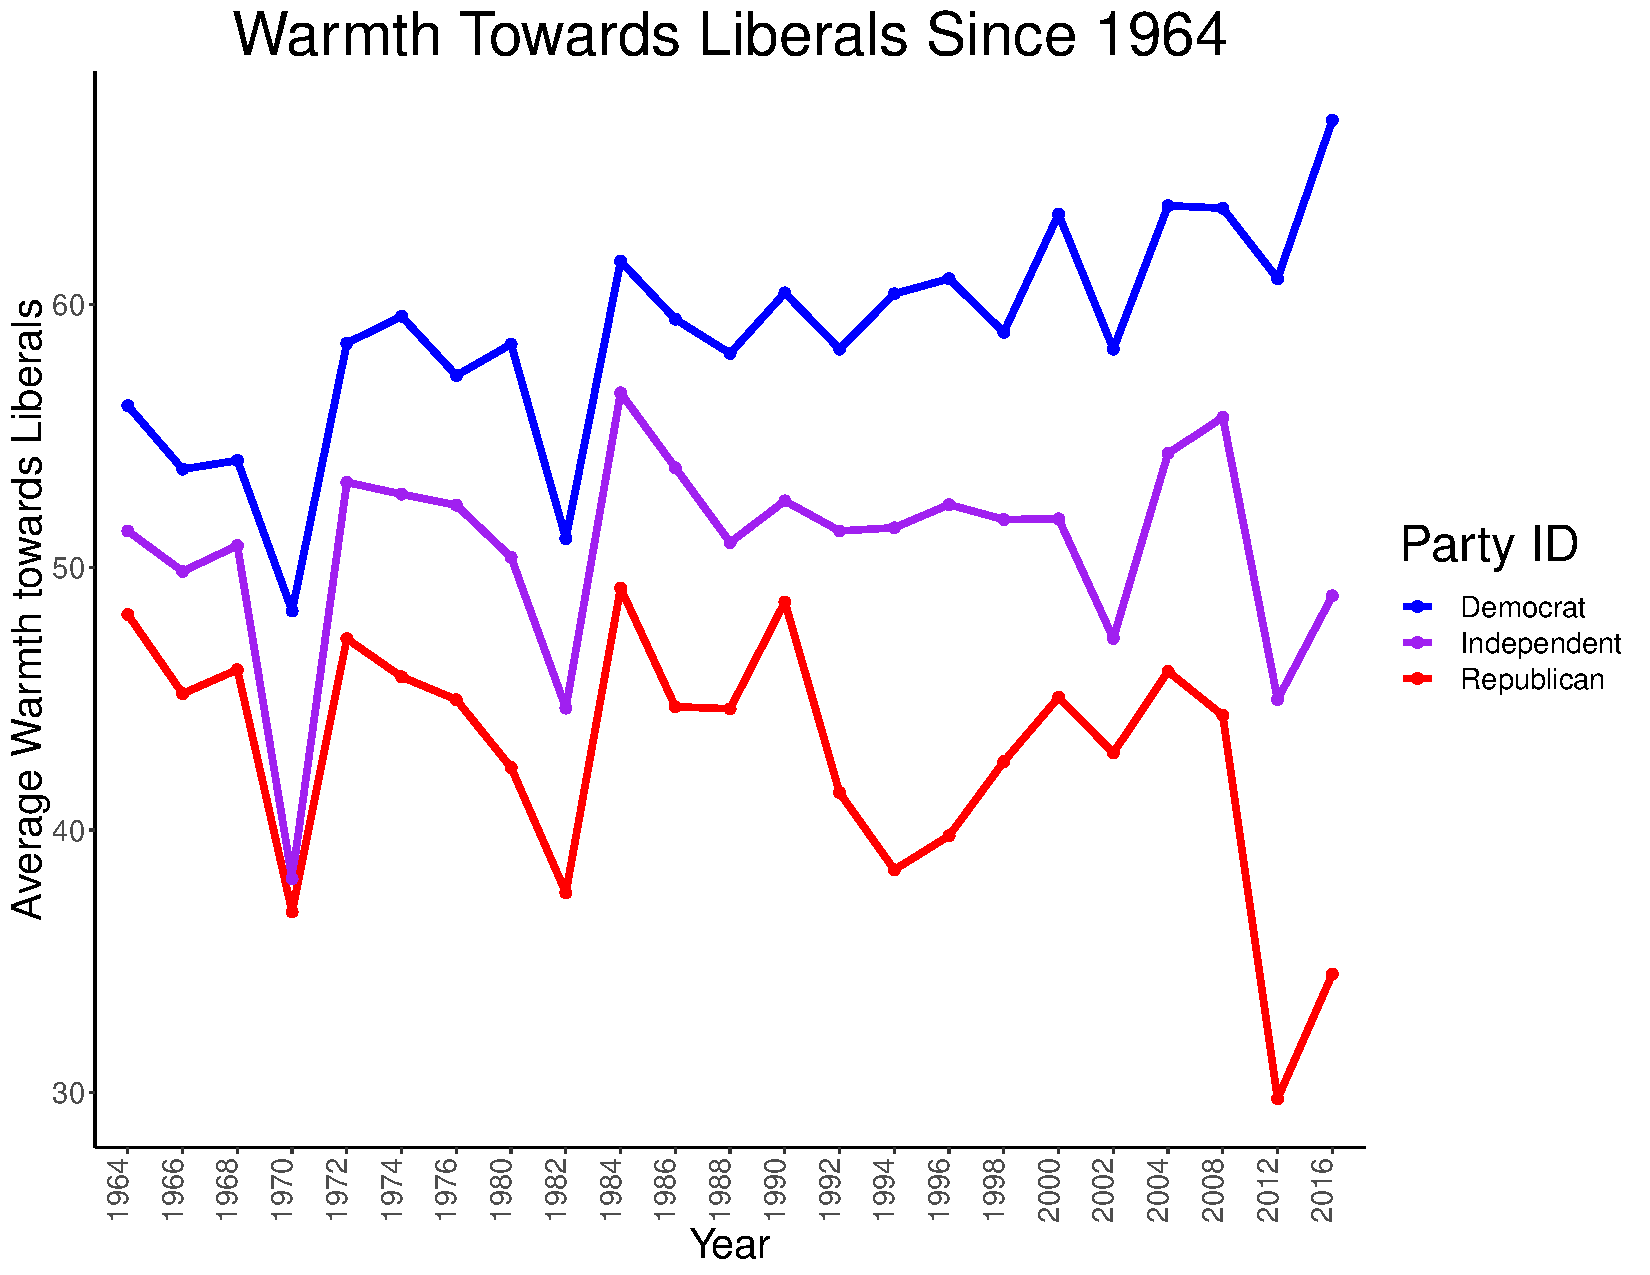
\includegraphics[width=.8\textwidth]{Liberals}}
	\end{figure}
\end{center}
\end{frame}

\begin{frame}
\frametitle{\ldots But we LIVE near each other}
\begin{center}
	\begin{figure}[ht!]  
		{	 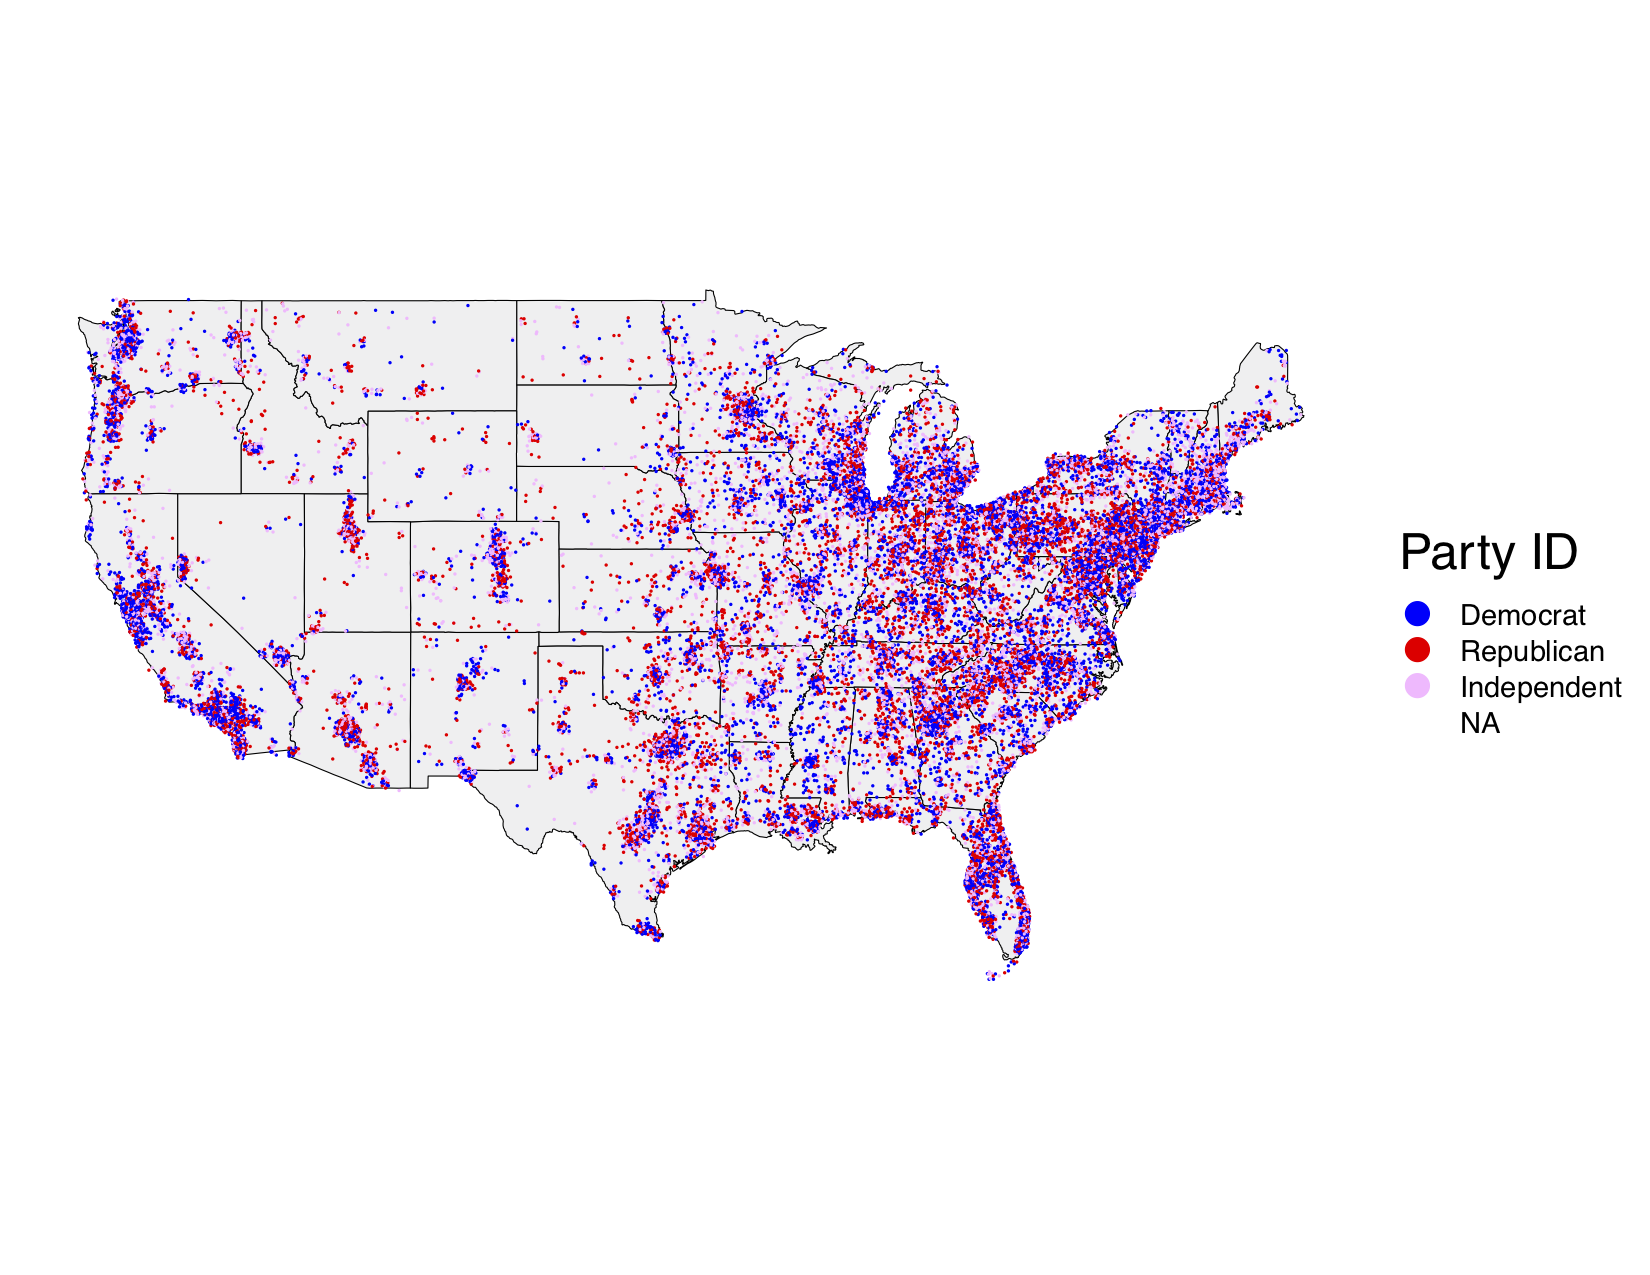
\includegraphics[width=\textwidth]{USMap}}
	\end{figure}
\end{center}
\end{frame}

\section{The Present Study}

\begin{frame}
\frametitle{What Causes How We Feel?}
\begin{enumerate}
	\item Our Knowledge?
	\item Our Participation?
	\item Our Groups?
	\item Some combination of the above?
\end{enumerate}
\end{frame}

\begin{frame}
\frametitle{Guiding Questions}
\begin{enumerate}
	\item Does political \tb{knowledge} influence feelings towards people in other parties or ideologies?
	\item Does political \tb{participation} influence feelings towards people in other parties or ideologies?
	\item Do knowledge and participation interact to influence feelings towards people in other parties or ideologies?
\end{enumerate}
\end{frame}


\section{Data Analysis}

\begin{frame}
\frametitle{Data}
\begin{center}
	\tb{American National Elections Studies}
	~~\\
	~~\\
	2016 Time Series Study
\end{center}
\end{frame}

\begin{frame}
\frametitle{Variables}
\begin{enumerate}
	\item \tb{IV:} Political Knowledge (0-5)
	\item \tb{IV:} Political Participation (0-11)
	\item \tb{PV:} Participant's Party ID and political ideology
	\item \tb{DV:} Feelings towards \ldots
	\begin{enumerate}
		\item Democrats
		\item Republicans
		\item Liberals
		\item Conservatives
	\end{enumerate}
\end{enumerate}
\end{frame}


\begin{frame}
\frametitle{Political Knowledge}
Who is...
\begin{enumerate}
	\item Joe Biden
	\item Paul Ryan
	\item Angela Merkel
	\item Vladimir Putin
	\item John Roberts
\end{enumerate}
\end{frame}

\begin{frame}
\small
\frametitle{Political Participation}
\begin{multicols}{2}
\begin{itemize}
	\item Talk to other about voting
	\item Go to political meeting
	\item Wear a campaign button
	\item Do other work for party
	\item Donate to campaign
	\item Donate to party
	\item Attend a rally/prtest
	\item Signed petition
	\item Posted on social media about politics
	\item Contact US Representative or Senator
	\item Voted in 2016
\end{itemize}
\end{multicols}	
\end{frame}

\begin{frame}
\frametitle{Feeling Thermometer}
\begin{center}
	Scale: 0 -- 100 
	~~\\
	~~\\
	Ratings between 50 degrees and 100 degrees  =  favorable and warm toward the party. 
	~~\\
	~~\\
	Ratings between 0 degrees and 50 degrees  = not favorable toward the person/don't care too much for that person.
\end{center}
\end{frame}

\begin{frame}
\frametitle{Plan for Analysis}
\begin{itemize}
	\item Correlation between knowledge and feeling DVs
	\item Correlation between participation and feeling DVs
	\item 2 (Knowledge: Less or More) $\times$ 3 (Participation: Less, Moderate, or More) ANOVA for each feeling DV
\end{itemize}
\end{frame}

\section{Results}

\begin{frame}
\frametitle{Correlation: Knowledge and Feelings}
\begin{center}
In general, the more we know does not yield more positive feelings towards each other.
\end{center}
\end{frame}

\begin{frame}
\begin{center}
	\begin{figure}[ht!]  
		{	 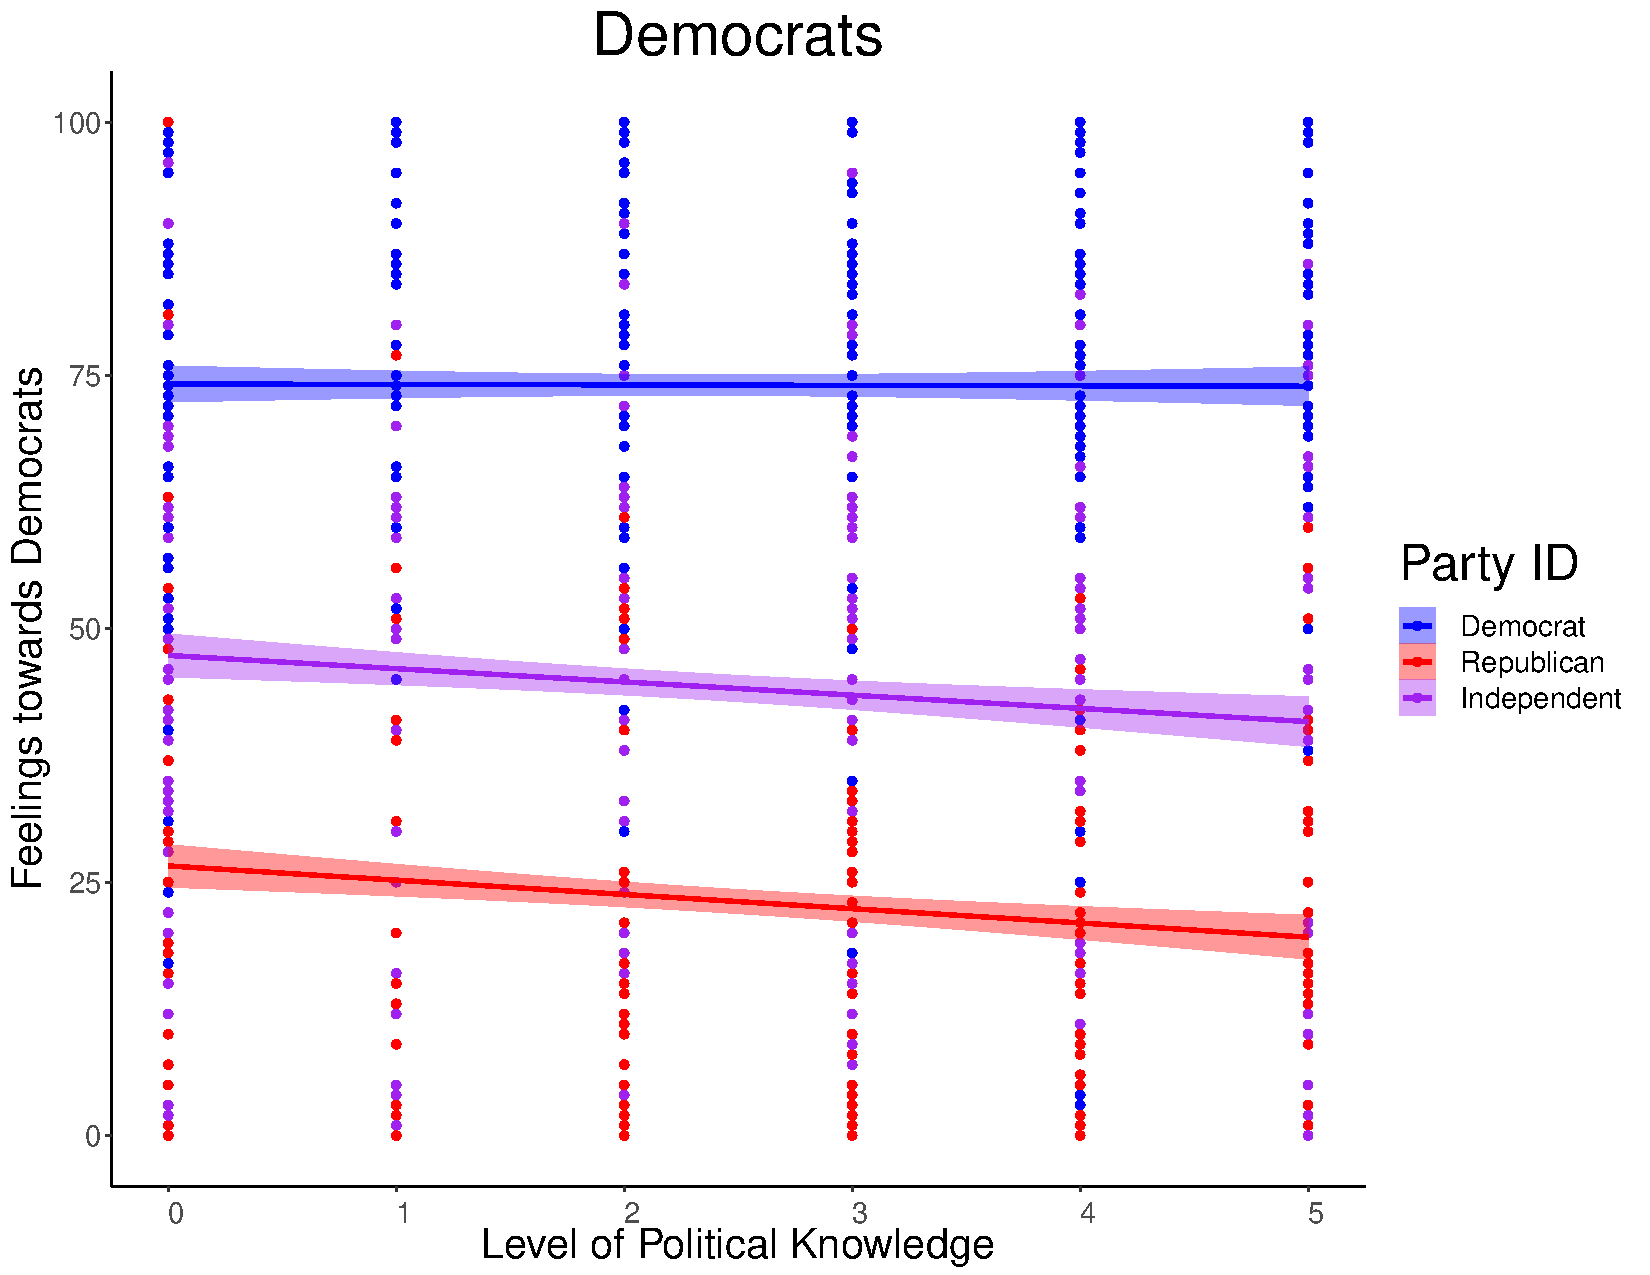
\includegraphics[width=.9\textwidth]{KFDem}}
	\end{figure}
\end{center}
\end{frame}

\begin{frame}
\begin{center}
	\begin{figure}[ht!]  
		{	 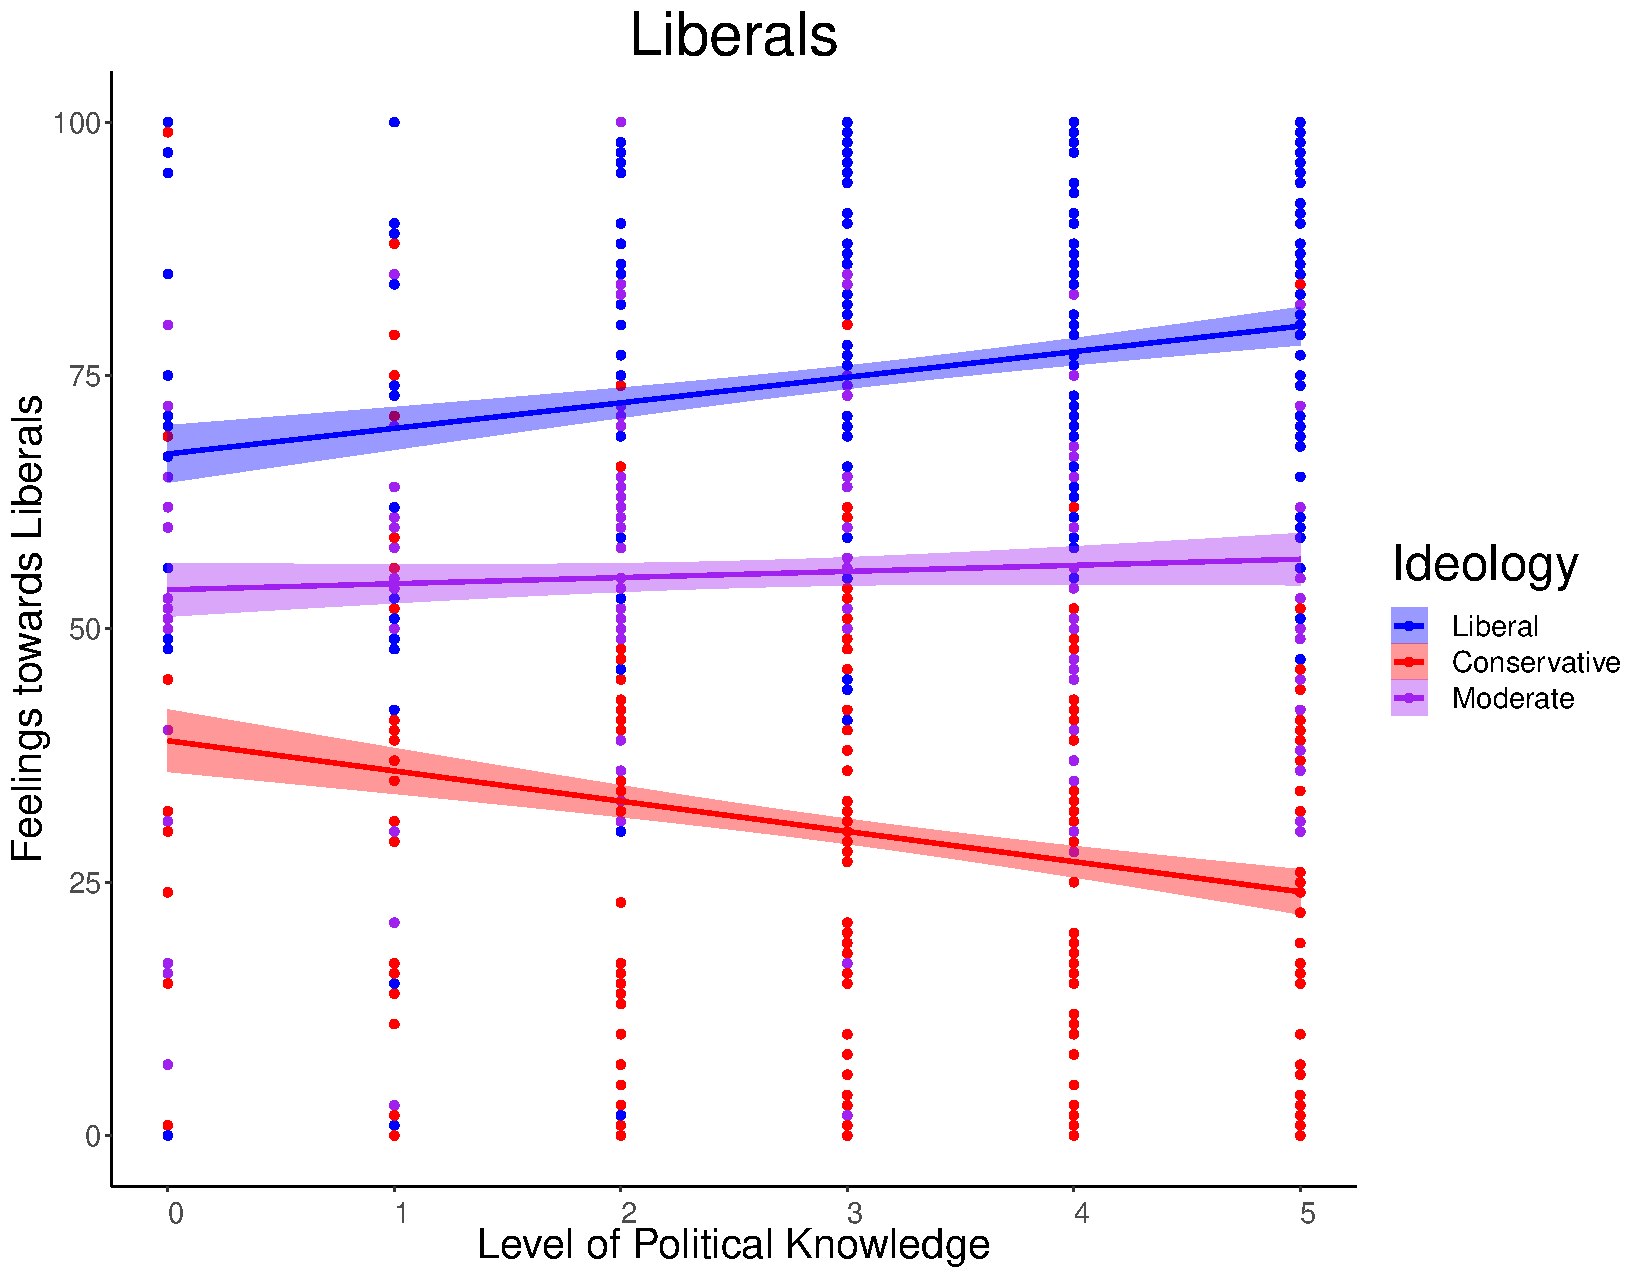
\includegraphics[width=.9\textwidth]{KFLib}}
	\end{figure}
\end{center}
\end{frame}

\begin{frame}
\frametitle{Correlation: Participation and Feelings}
\begin{center}
	In general, the more we participate does not yield more positive feelings towards each other.
\end{center}
\end{frame}


\begin{frame}
\begin{center}
	\begin{figure}[ht!]  
		{	 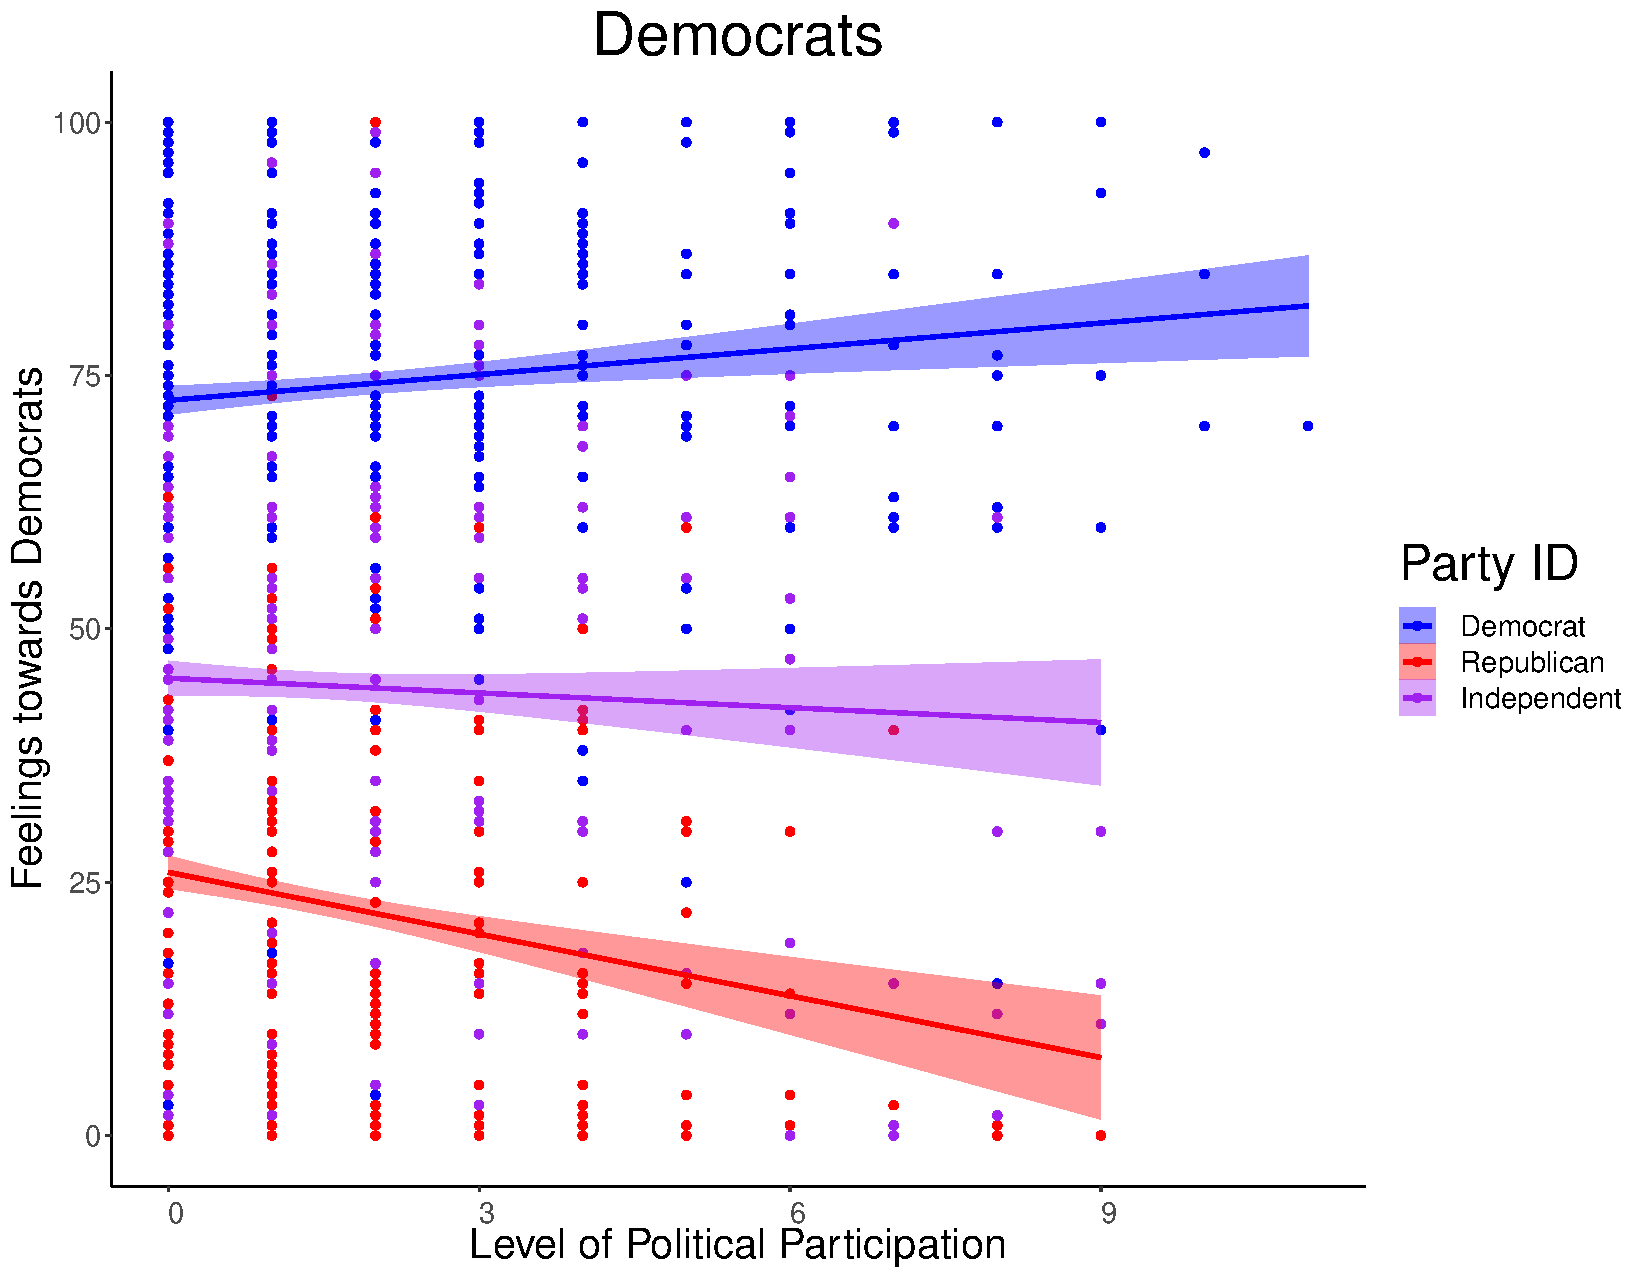
\includegraphics[width=.9\textwidth]{PFDem}}
	\end{figure}
\end{center}
\end{frame}

\begin{frame}
\begin{center}
\begin{figure}[ht!]  
	{	 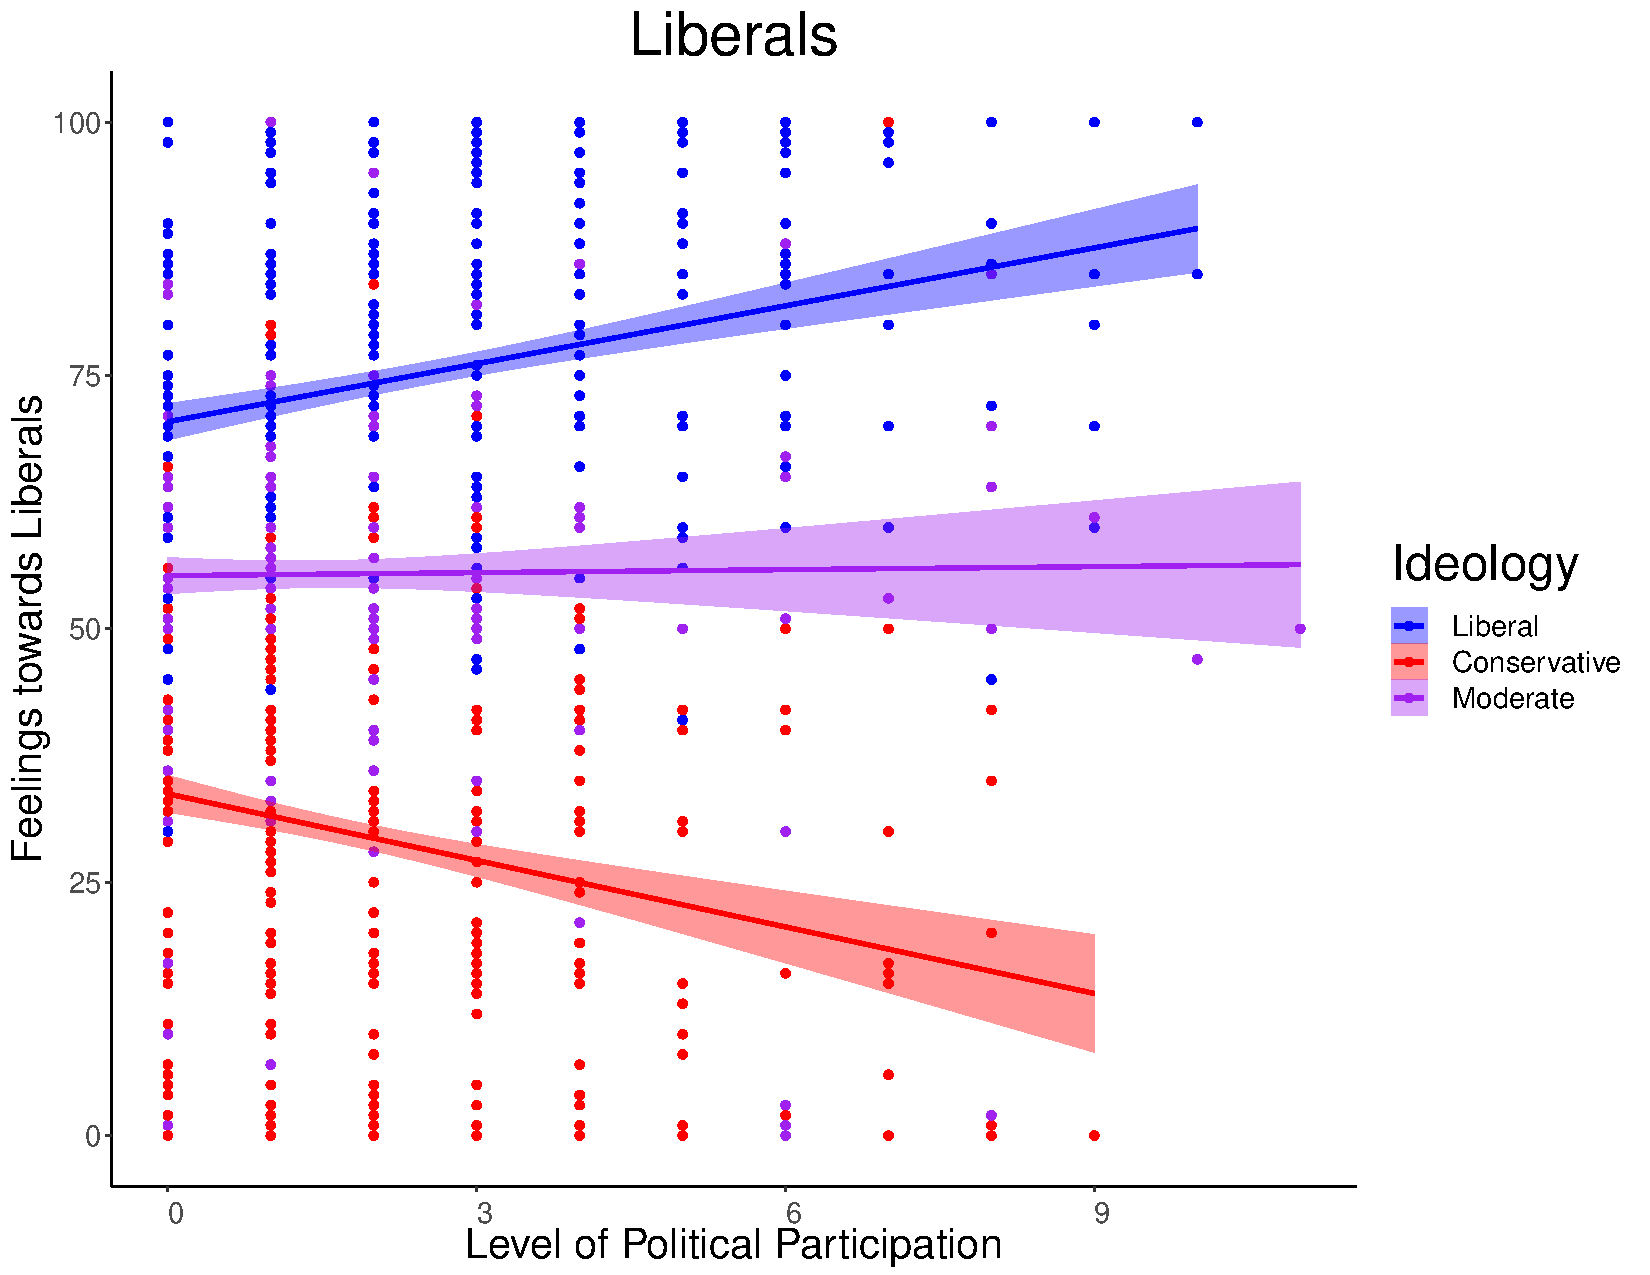
\includegraphics[width=.9\textwidth]{PFLib}}
\end{figure}
\end{center}
\end{frame}

\begin{frame}
\frametitle{ANOVA: Knowledge $\times$ Participation}
\begin{enumerate}
	\item For feelings towards parties: There is a main effect of participation and a main effect of knowledge but no interaction
	\item For feelings towards ideologies: There is a main effect of participation, but no main effect of knowledge and no interaction
\end{enumerate}
\end{frame}

\begin{frame}
\begin{center}
	\begin{figure}[ht!]  
		{	 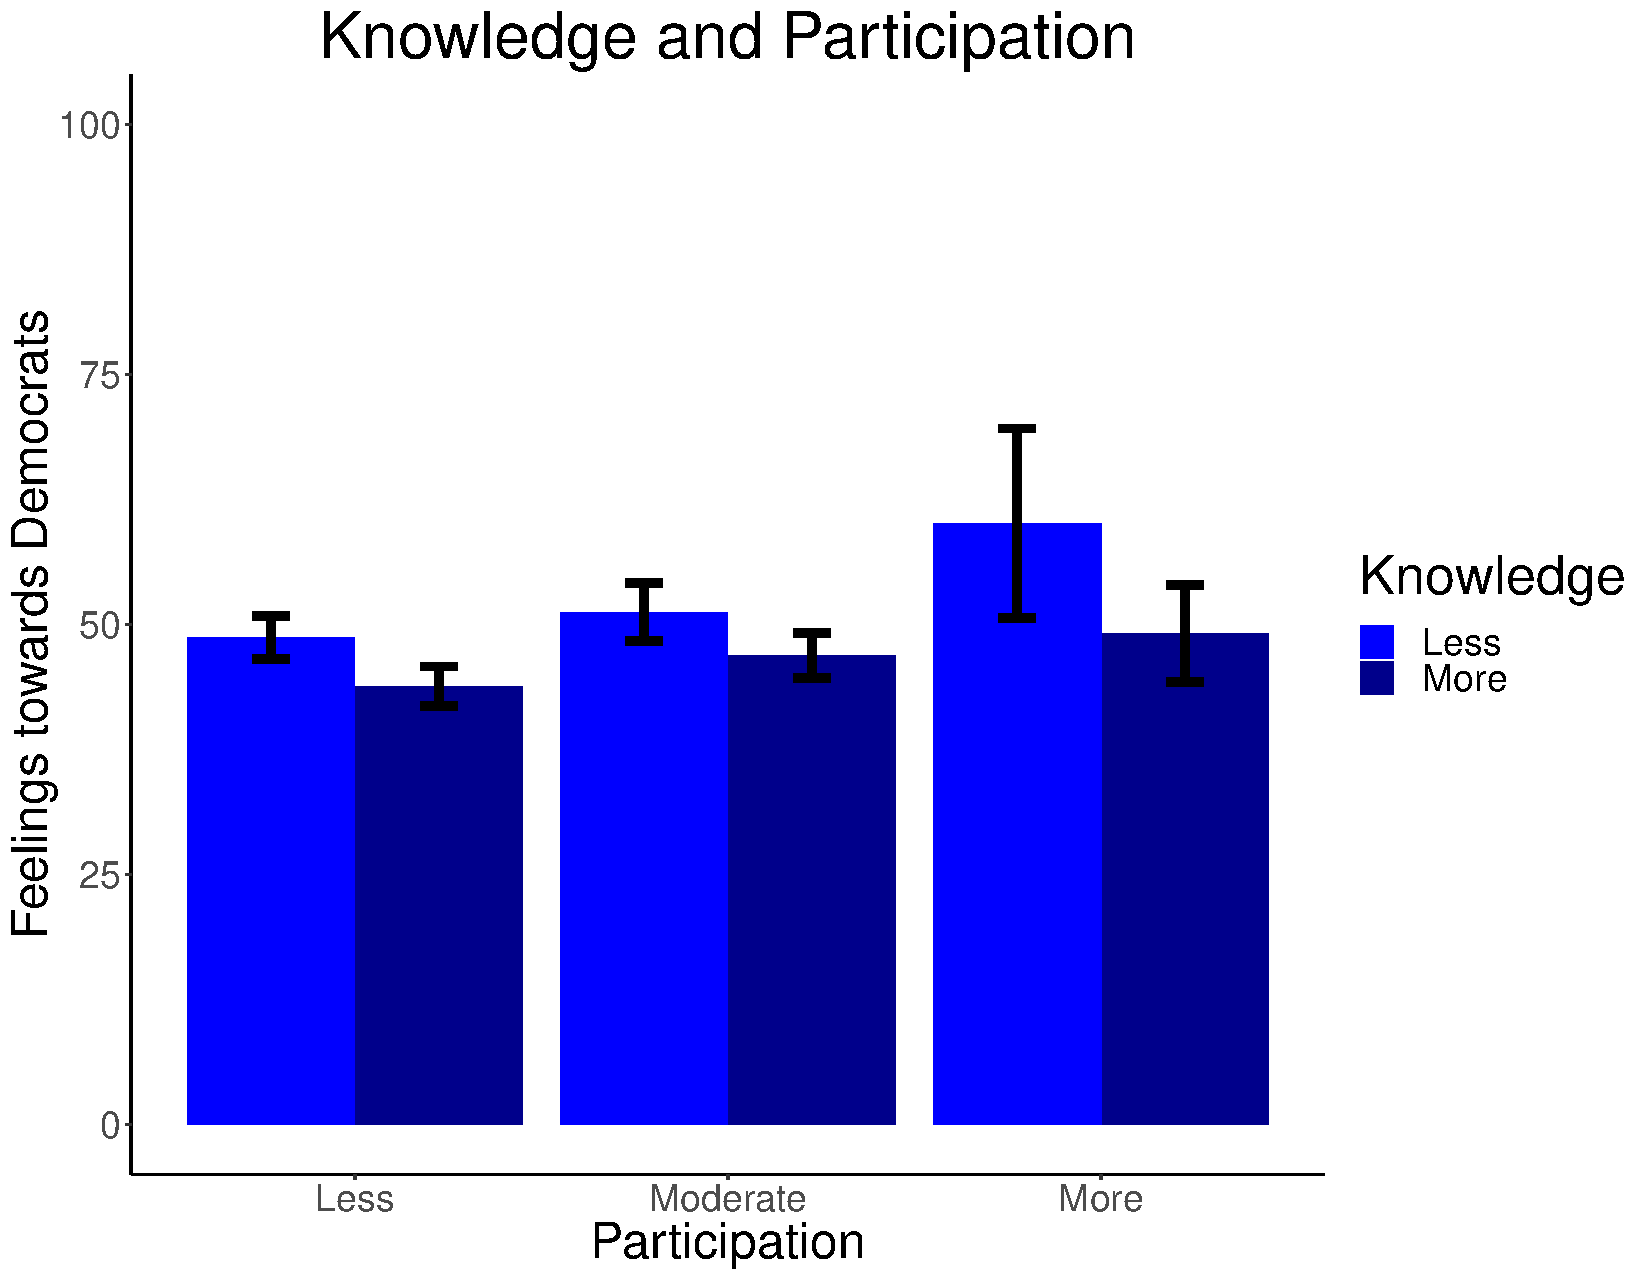
\includegraphics[width=.9\textwidth]{KPDem}}
	\end{figure}
\end{center}
\end{frame}

\begin{frame}
\begin{center}
\begin{figure}[ht!]  
	{	 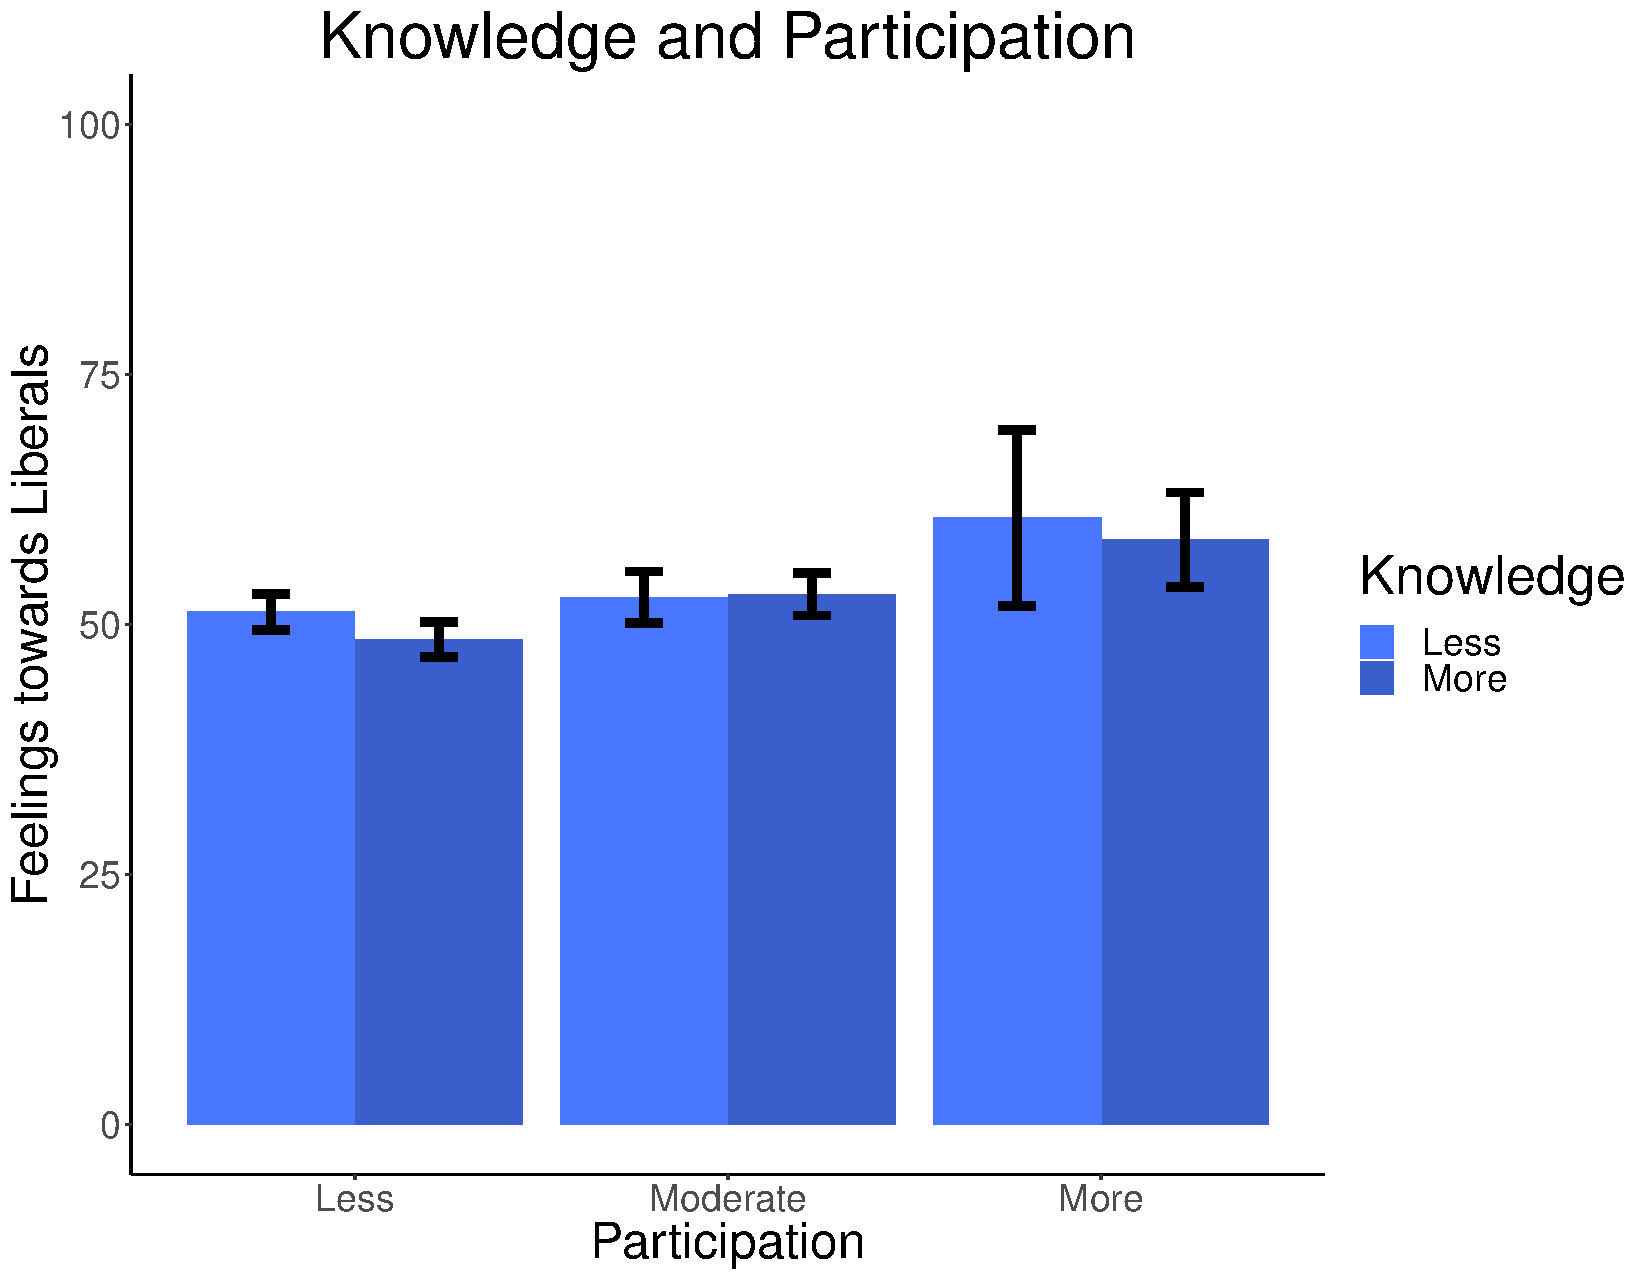
\includegraphics[width=.9\textwidth]{KPLib}}
\end{figure}
\end{center}
\end{frame}

\begin{frame}
\frametitle{ANOVA: Knowledge $\times$ Participation (continued)}
Break the analysis down by parties and ideologies becomes more tricky
\end{frame}

\begin{frame}
\begin{center}
	\begin{figure}[ht!]  
		{	 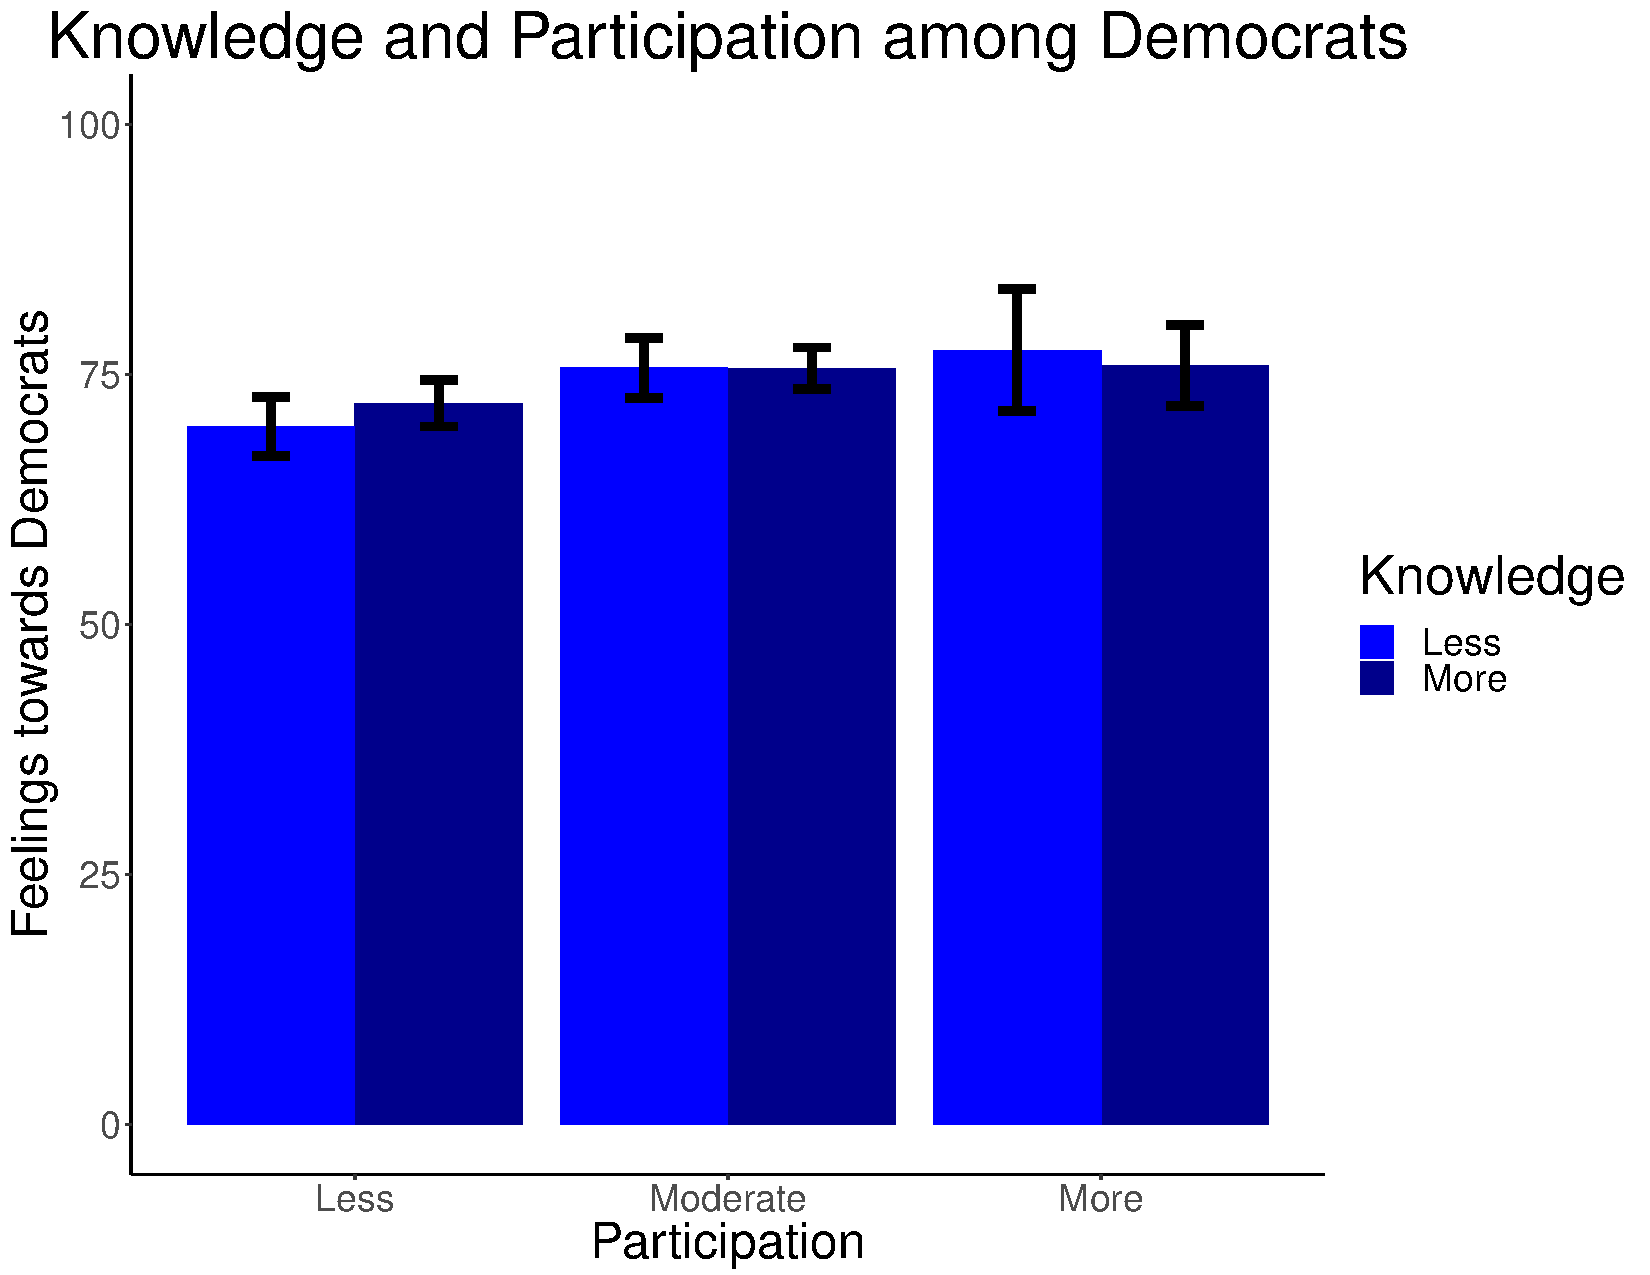
\includegraphics[width=.9\textwidth]{KPDemADem}}
	\end{figure}
\end{center}
\end{frame}

\begin{frame}
\begin{center}
	\begin{figure}[ht!]  
		{	 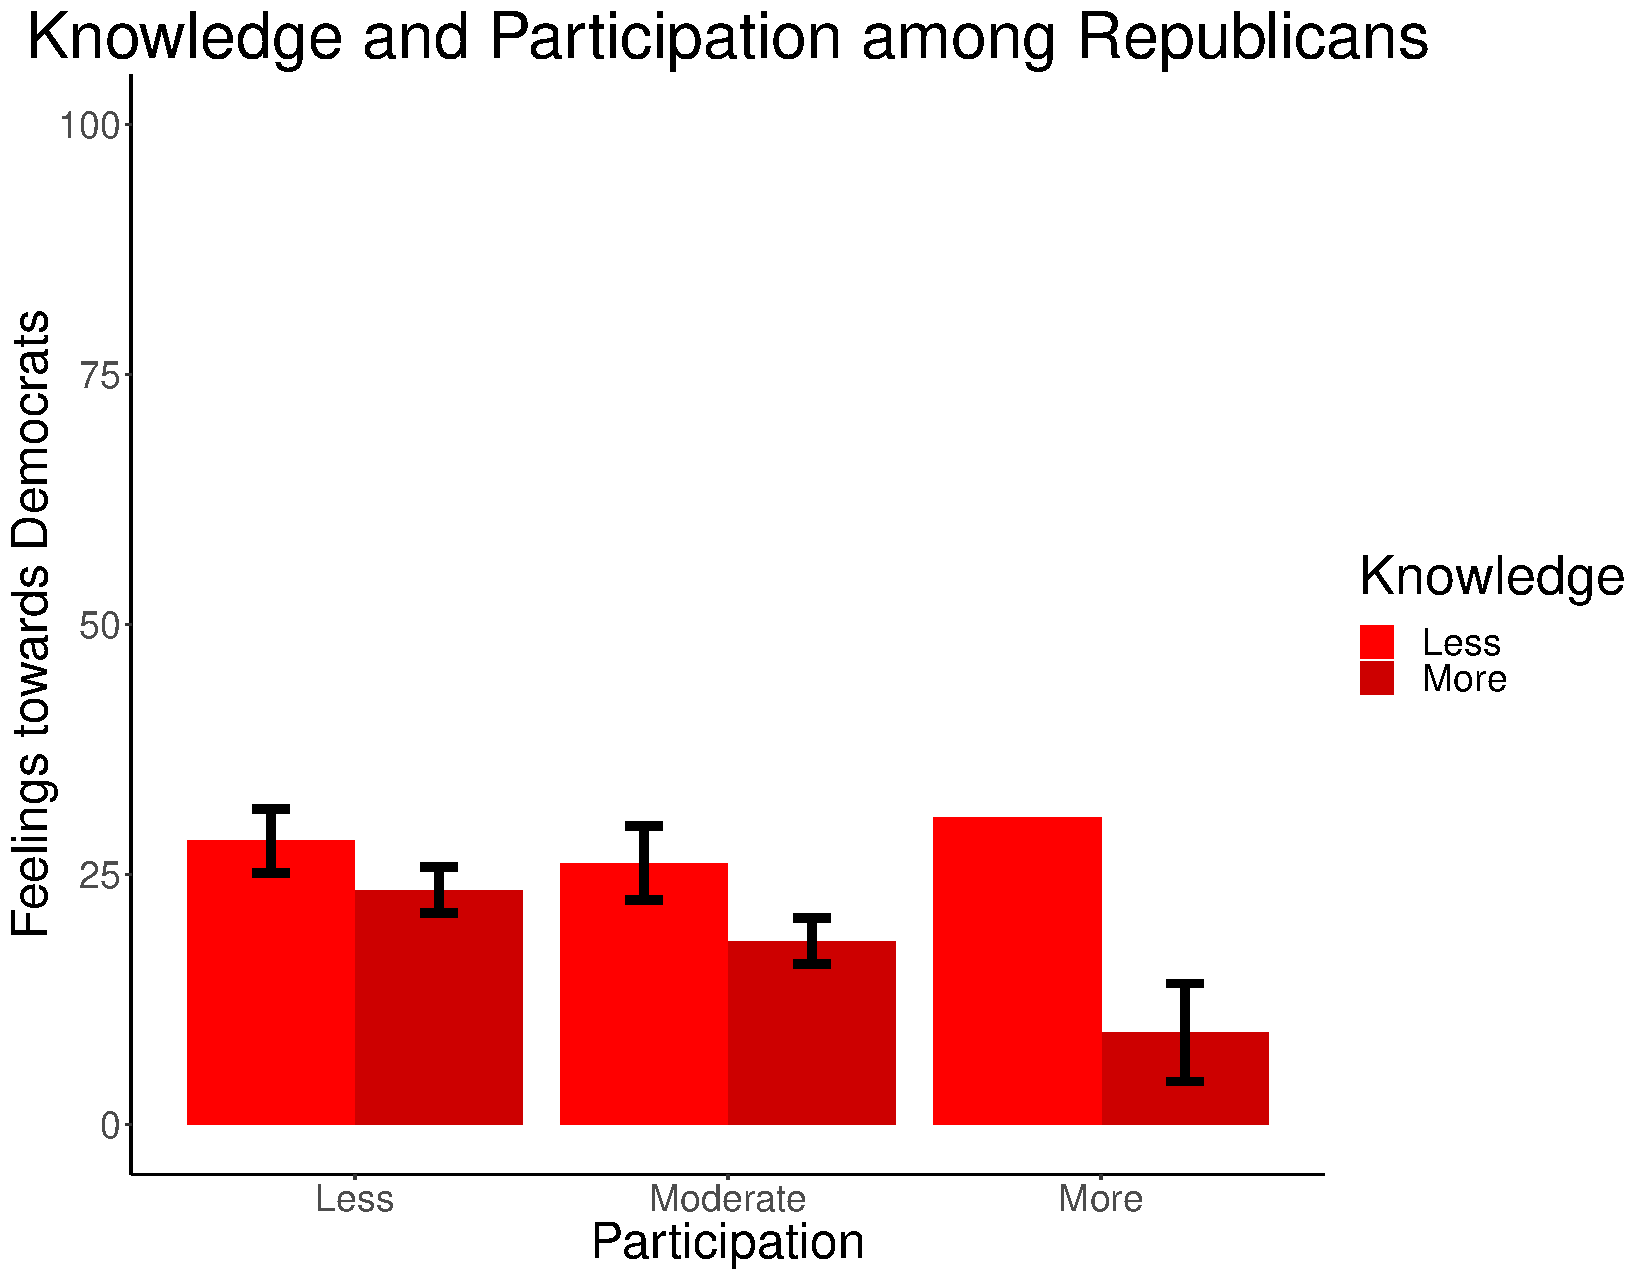
\includegraphics[width=.9\textwidth]{KPDemARep}}
	\end{figure}
\end{center}
\end{frame}

\begin{frame}
\frametitle{Conclusions}
\begin{enumerate}
	\item Knowledge and Participation individually influence feelings towards parties and ideologies
	\item \e{However}, affective relationships towards parties and ideologies are better predict partisan and ideological feelings
\end{enumerate}
\end{frame}

\begin{frame}
\frametitle{Future Directions: Affect Over Action?}
\begin{center}
	\begin{figure}[ht!]  
		{	 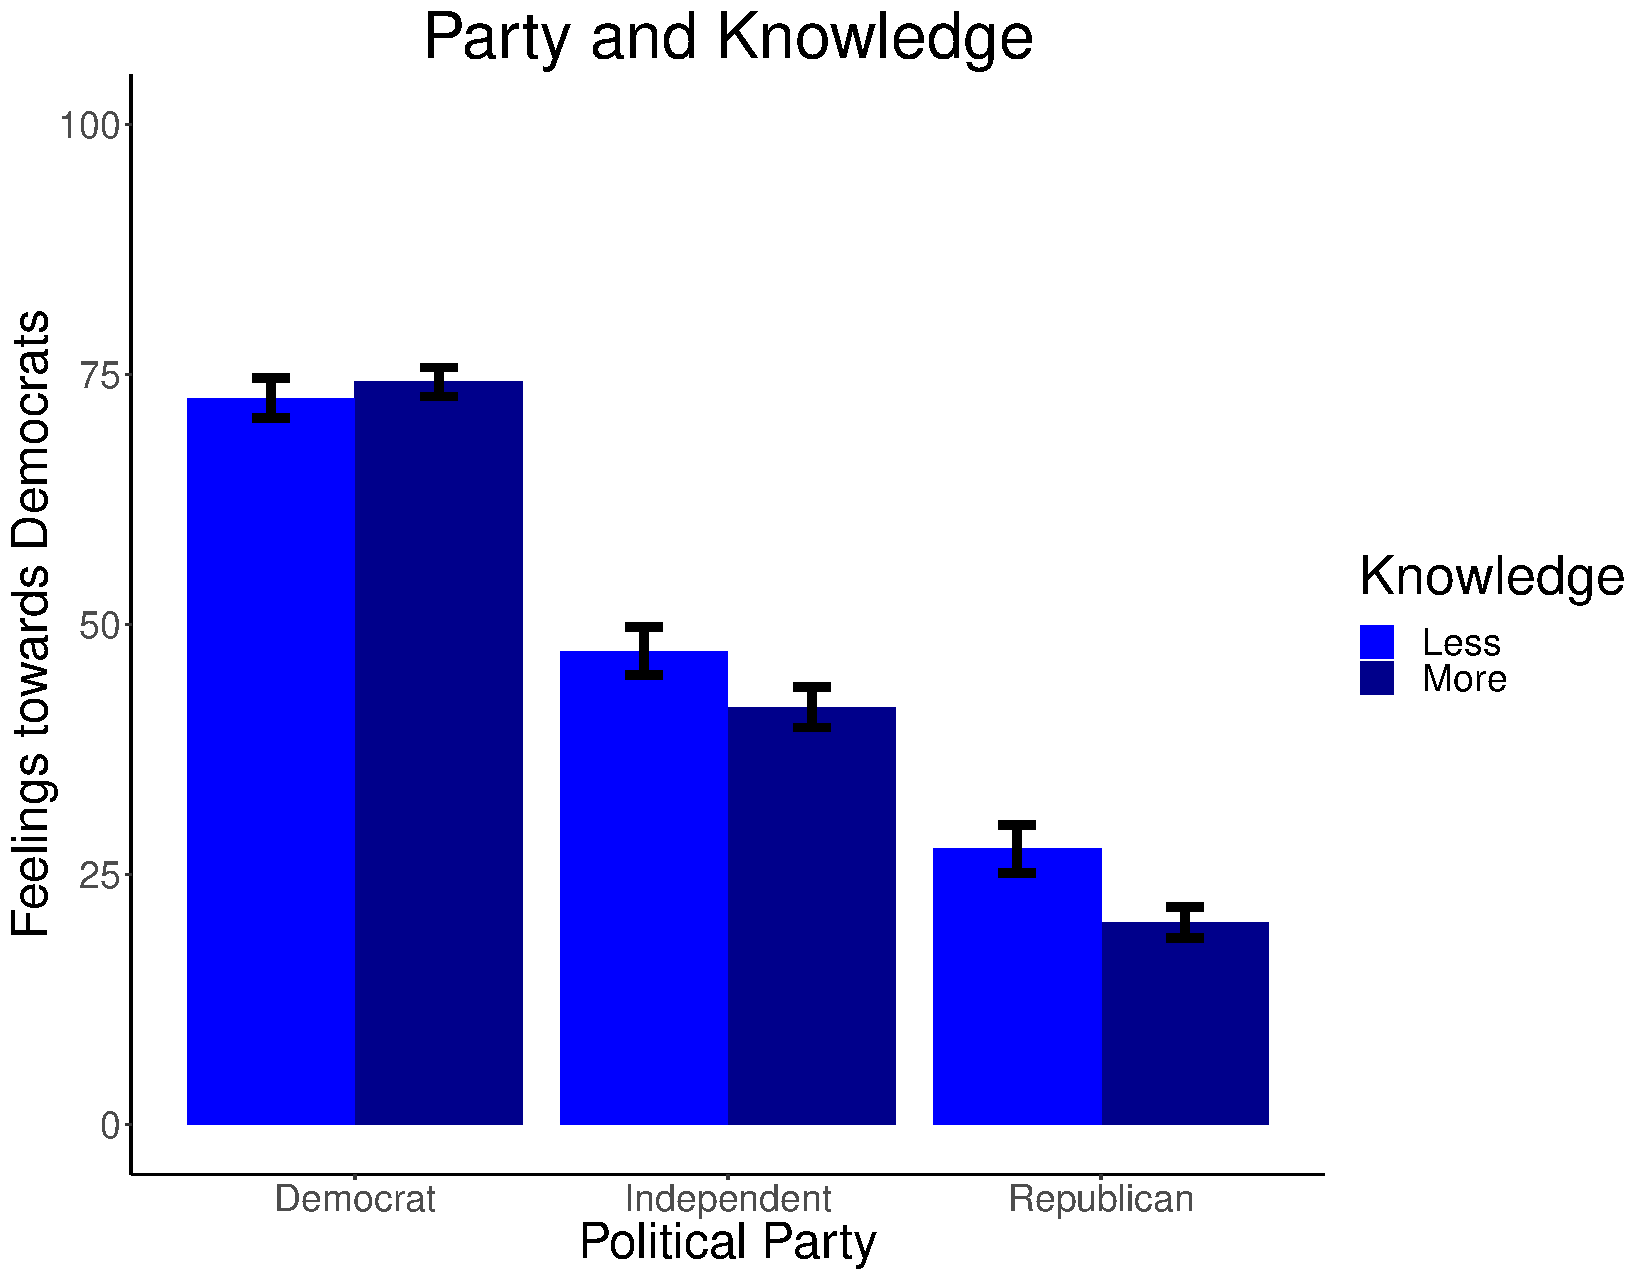
\includegraphics[width=.8\textwidth]{KnowPartyDem}}
	\end{figure}
\end{center}
\end{frame}

\begin{frame}
\frametitle{Replication Materials}
\begin{center}
	\url{https://github.com/lin-jennifer/Political-Prejudice}
	
~~\\
Software Requirements: \tb{R Studio} and \LaTeX

\end{center}
\end{frame}

\end{document}